\documentclass{report}
\usepackage{graphicx}
\usepackage{xeCJK}
\usepackage{pgfplots}
\pgfplotsset{compat=1.18}
\setCJKmainfont{Hiragino Mincho ProN} % Macの日本語フォント

\begin{document}

\chapter{レポートのタイトル}

\section{画像}
図\ref{fig:sample}はサンプル画像を示しています。
\begin{figure}[htbp]
  \centering
  
\includegraphics[width=0.7\textwidth]{Its_me.jpg}
  \caption{サンプル画像}
  \label{fig:sample}
\end{figure}

\section{表}
表\ref{tab:sample}はデータの一覧を示しています。
\begin{table}[htbp]
  \centering
  \caption{サンプル表}
  \begin{tabular}{|c|c|c|}
    \hline
    項目 & 数値 & 備考   \\
    \hline
    A  & 10 & データA \\
    B  & 20 & データB \\
    C  & 30 & データC \\
    \hline
  \end{tabular}
  \label{tab:sample}
\end{table}

\section{二次関数のグラフ}
図\ref{fig:quadratic}は二次関数 $y = x^2$ のグラフです。
\begin{figure}[htbp]
  \centering
  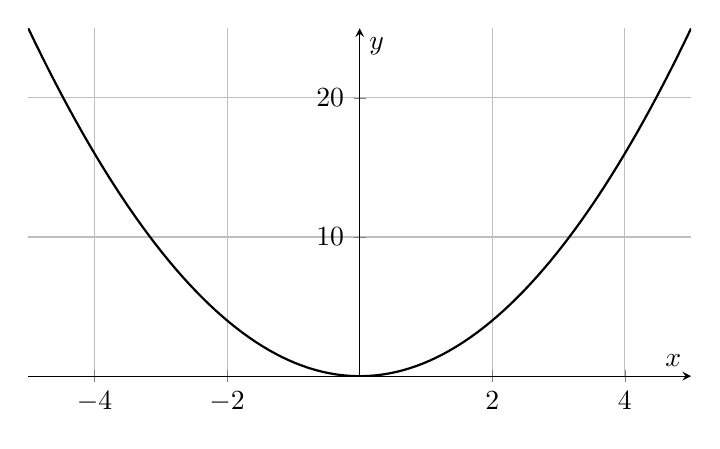
\begin{tikzpicture}
    \begin{axis}[
        axis lines = middle,
        xlabel = $x$, ylabel = $y$,
        grid = both,
        samples = 100,
        width=10cm, height=6cm
      ]
      \addplot[domain=-5:5, thick] {x^2};
    \end{axis}
  \end{tikzpicture}
  \caption{二次関数 $y = x^2$ のグラフ}
  \label{fig:quadratic}
  \cite{einstein1905}
\end{figure}

\section{参考文献}
\begin{thebibliography}{9}
  \bibitem{einstein1905}
  Albert Einstein,
  \textit{Zur Elektrodynamik bewegter Körper},
  Annalen der Physik, 17 (1905), pp. 891–921.
\end{thebibliography}

\end{document}